\section{Data Integration and Assimilation Systems}
\label{se:dias}

\acrfull{dias} collects and files data from satellites, ground observation stations, numerical weather prediction models and climate change projection models. Once this data is integrated with geographic and socio-economic information, DIAS generates results for managing global environmental issues and natural disasters \cite{Kawasaki2018DataReduction}. As mentioned above, \acrshort{dias} has the capability of collecting weather data form multiple data sources which are inherently in different formats. After successfully ingest the data, it generate results which can use for different kind of purposes.

\begin{figure}[htp]
    \centering
    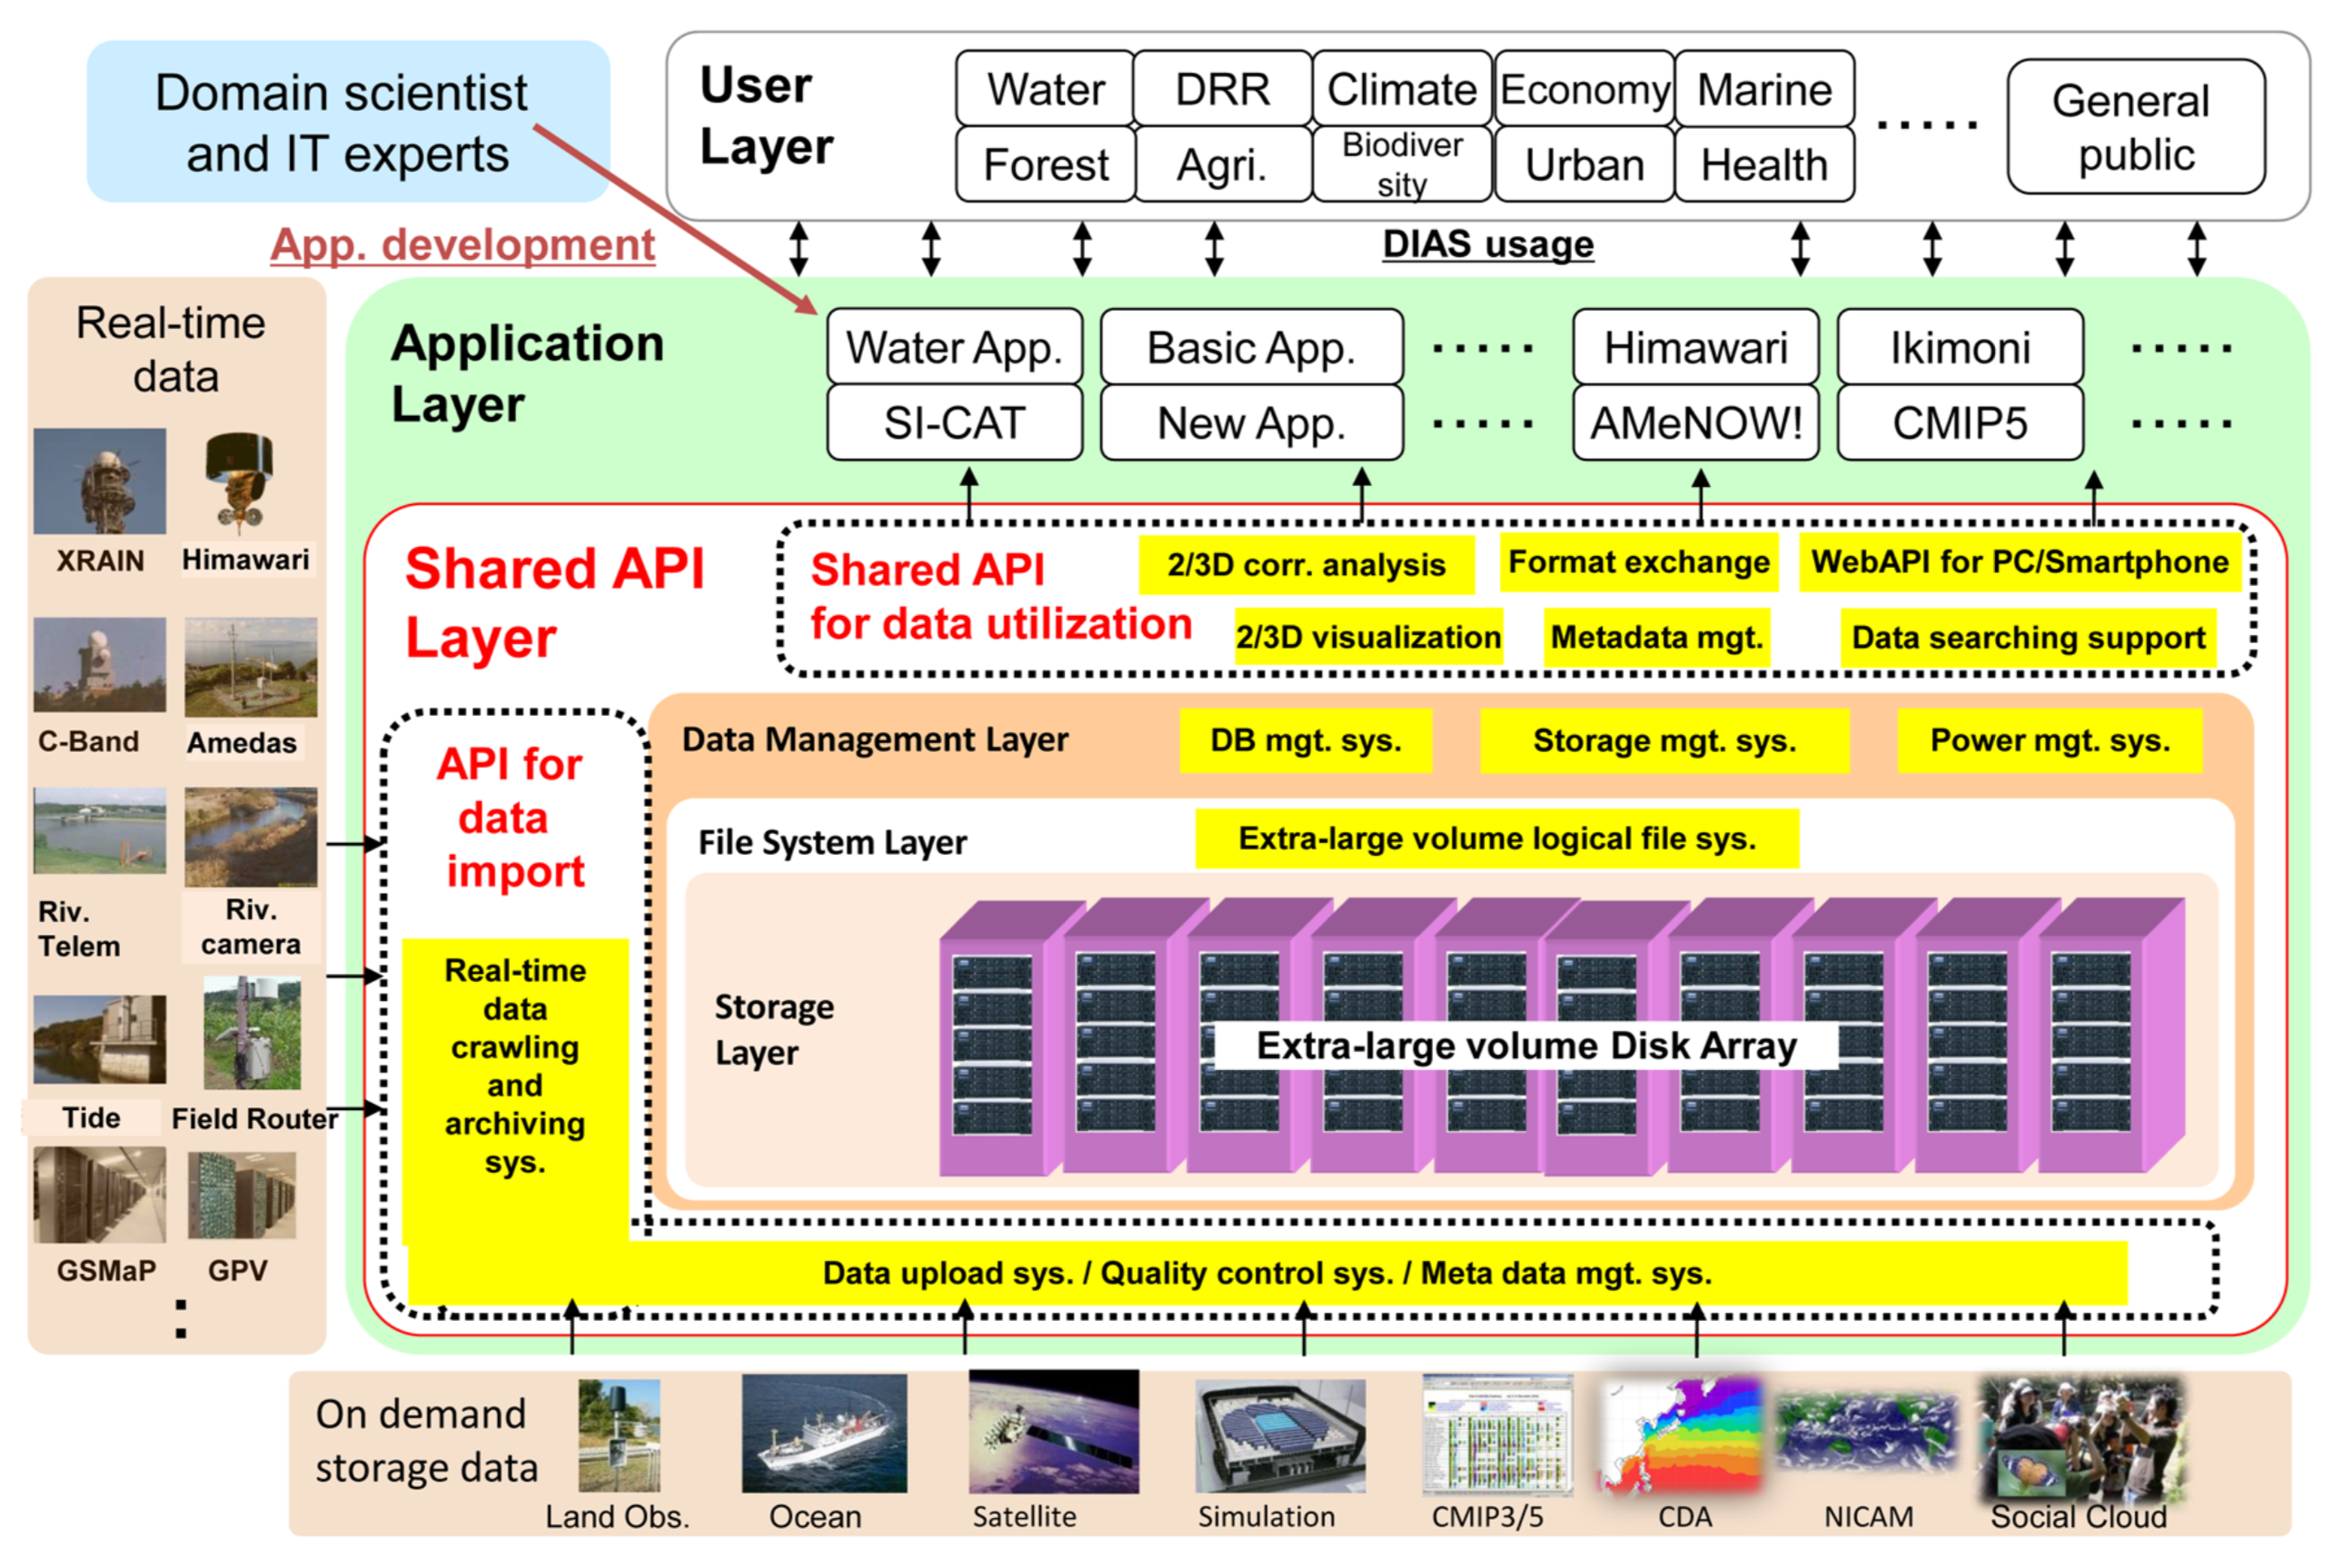
\includegraphics[width=1\textwidth]{lit/other/dias_common_base_application_platform.png}
    \caption[DIAS’s common base application platform.]{DIAS’s common base application platform \cite{Kawasaki2018DataReduction}.}
    \label{fi:dias_common_platform}
\end{figure}

The mechanism of storing data in \acrshort{dias}, similar to the other systems discussed.
These data sets are stored in an extra large volume disk array system with API (Application Programming Interface) software used to import the data. APIs work to convert or re-format data into manageable forms and are useful in creating the DIAS storage archive. API software consists of several tools, including the real-time data crawling and archiving system, data upload system, quality control system, and metadata management system \cite{Kawasaki2018DataReduction}. To store on the large volume of disk space, it convert the data via provided set of APIs. This can be consider same as the open data model provide by the \acrshort{fews}. Other than that, \acrshort{dias} consist of additional tools which provide the functionality of quality control of the data, and metadata management which is similar to some of services in \acrshort{lead}.

As shown in \cref{fi:dias_common_platform}, it provides an application layer which allows domain scientists to working on research tasks, and to develop specific tools and applications by working together with Information Technology experts \cite{Kawasaki2018DataReduction}. Once the data is achieved on the \acrshort{dias} system, it share those details via Shared API layer. Thus it allows users to remote access to the data, and easy integration via the APIs.



%%%%%%%%%%%%%%%%%%%%%%%%%%%%%%%%%%%%%%%%%%%%%%%%%%%%%%%%%%%%%%%%%%%%%%%%%%%%%%%%
\section{Meteorological Assimilation Data Ingest System}
\label{se:madis}
\acrfull{madis} is a data ingest and assimilation system, which is collecting data over dozen of providers, then quality control over the data and store in \acrshort{netCDF} format. Later allow users to access the data via supporting different type of protocols.

\begin{figure}[htp]
    \centering
    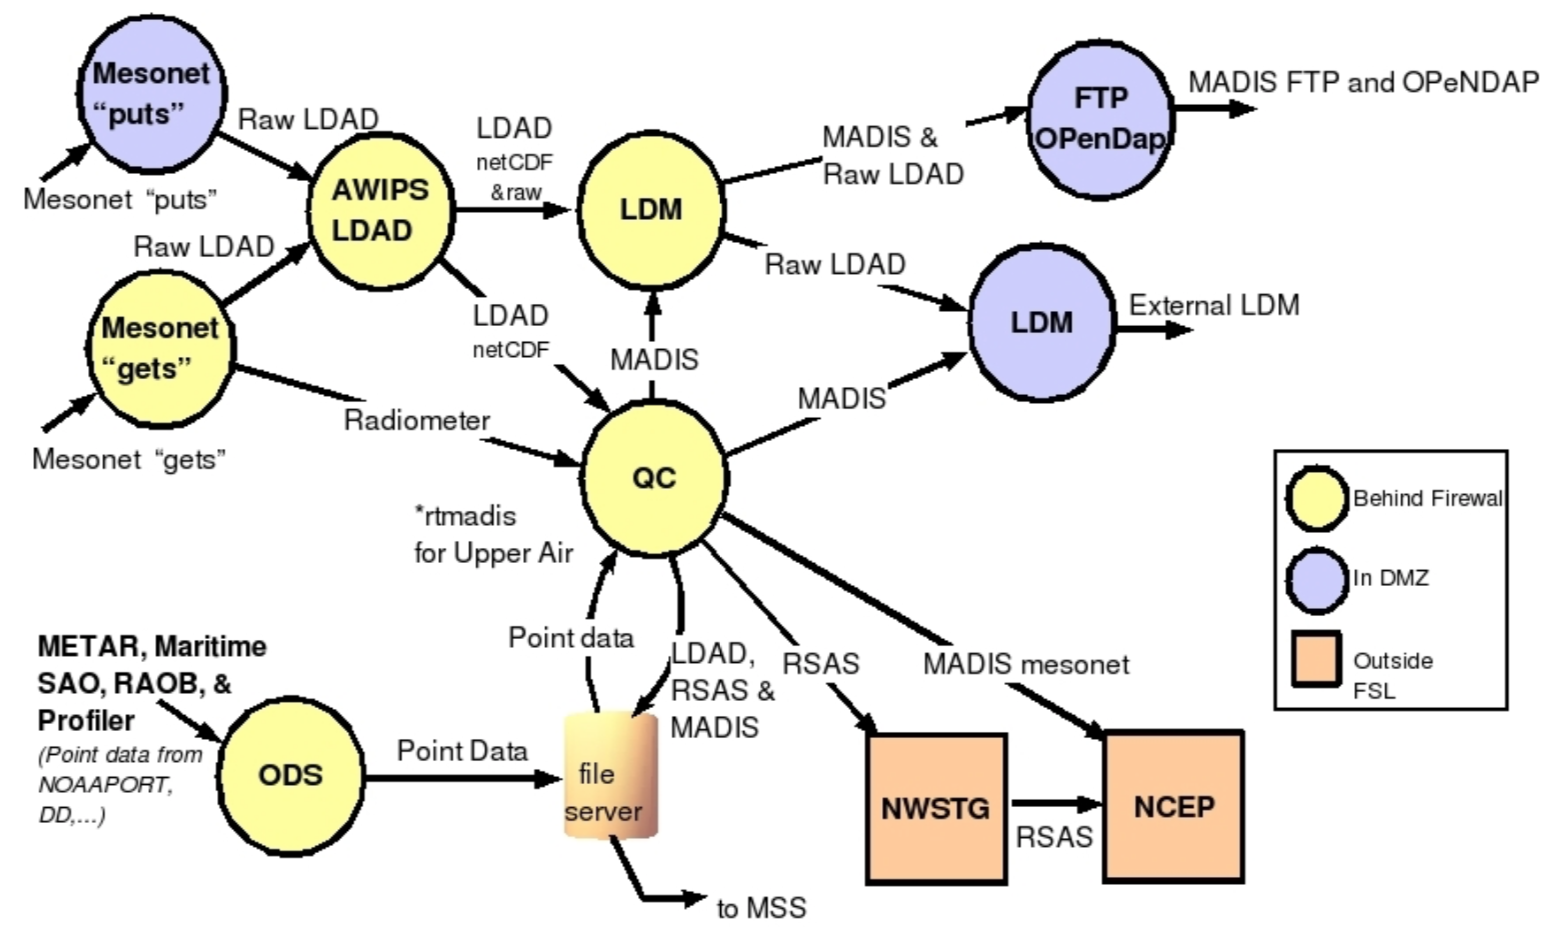
\includegraphics[width=1\textwidth]{lit/other/madis_flow.png}
    \caption[\acrshort{madis} flow]{\acrshort{madis} flow \cite{Macdermaid2005ARCHITECTUREP2.39}.}
    \label{fi:madis_flow}
\end{figure}

\dbc{In Fig. 2.8, is it the data flow?}
\gkc{The paper is not very much clear. I think it shows data flow with including some of it integration functions.}

\acrshort{madis} comprises a distributed architecture for ingest, processing, and data distribution functions.
In addition, in a recent architectural advance, the various functional hosts are arranged in pairs using High-Availability (HA) Linux to provide auto mated failover in case of system failure. Real-time data distribution methods include FTP, Local Data Manager (LDM), and the Web-based OPeNDAP (OPen source project for Network Data Access Protocol) \cite{Macdermaid2005ARCHITECTUREP2.39}. As it mentioned above, the \acrshort{madis} is implemented based on a distributed architecture which is available at the time of it's development. Even it is not clear mentioned, it is using functional call like Remote Procedure Call (RPC) to invoke among a cluster of nodes. In \cref{fi:madis_flow}, data are transported from input and preprocessing systems to the central compute systems and then out to other hosts for storage and distribution \cite{Macdermaid2005ARCHITECTUREP2.39}. To get high availability, it has added some update to it's architecture as mentioned in the paper. The conclusion of this statement is, these kind of functionalities are available at the modern the Cloud Computing tools, and out of the box those tools are providing the scalability and high availability. Using those tools, it possible to implement a such system with less effort and high confidence.

MADIS routinely acquires mesonet data from several dozen network providers representing over 14,000 stations. This translates into over 30,000 station reports each hour. Several systems running both inside and outside the firewall acquire the data. These data are sent to the Central Facility's Advanced Weather Interactive Processing System (AWIPS) data server for preprocessing and conversion to a common format, NetCDF. The NetCDF files are then transferred to the MADIS compute nodes \cite{Macdermaid2005ARCHITECTUREP2.39}. This provide an overview of the level of data that \acrshort{madis} handling. This could be a good reference for implementing \acrshort{wdias}, and it's performance testing. As same as \acrshort{fews}, it is also converting the data into a common format which is \acrshort{netCDF}. Those files are transferred to the computer nodes, and allow users to access via OPeNDAP.

The MADIS compute platforms comprise Intel based servers running the Red Hat Enterprise Linux operating system. Many of these computers are configured using High-Availability Linux clustering \cite{Macdermaid2005ARCHITECTUREP2.39}. As it indicated above, the system is heavily depend on the platform. There is a cost involving purchasing those license.

Since some MADIS data are considered proprietary by the provider, access to these data need to be controlled. To accommodate this, MADIS data are split into six different versions based on the level of access allowed by the data provider \cite{Macdermaid2005ARCHITECTUREP2.39}. When compared to \acrshort{fews}, \acrshort{madis} provide a control based access to the data.



%%%%%%%%%%%%%%%%%%%%%%%%%%%%%%%%%%%%%%%%%%%%%%%%%%%%%%%%%%%%%%%%%%%%%%%%%%%%%%%%
\section{Summary}
\label{se:lit_summary}
Several related work that discussed above in this chapter, mainly focus on issue of storing data which are ingest from different sources with different formats efficiently. The \acrshort{fews} and \acrshort{madis} are using the \acrshort{netCDF} as the common data format to store the data which is one of best solution available with modern technologies as well. Even it is not clearly mentioned, the \acrshort{dias} and \acrshort{lead} also following a method of having common storage space in order to store bulk data.
\acrshort{fews} and \acrshort{lead} have the capability of handling workflow of forecasting, but other system are mainly focus on providing a weather data management system.
\acrshort{fews} provide a modular approach via it's general adapter which is shown on \cref{fi:fews_general_adapter}, and according to the \acrshort{soa} architecture of \acrshort{lead} provide the same functionality via services.

Most of the above systems develop by many developers and researcher via many of funding. And most of them are depend on underline platform, and not up to date with the modern technologies such as cloud computing.
